\section{GUI}
	\begin{frame}{GUI: Introduction}
		\begin{itemize}
			\pause
			\item The graphical user interface is an optional feature so the scientists can easily use MOAB Workload Manager and dynamic scheduler interface. 
			\pause
			\item The user can generate a shell script for MOAB Workload Manager and send it via SSH to the server.
			\pause
			\item User can also discover relationships in his/her tasks and observe the performance the program. 
			
		\end{itemize}
	\end{frame}
	
	\begin{frame}{GUI: Architecture}
		\begin{itemize}
			\item The main architecture pattern, the graphical user interface is oriented to, is the Model-View-
Presenter. 
	        \item The view of the user interface is developed in the FXML scripting language and Java code is used for application logic.
	        
				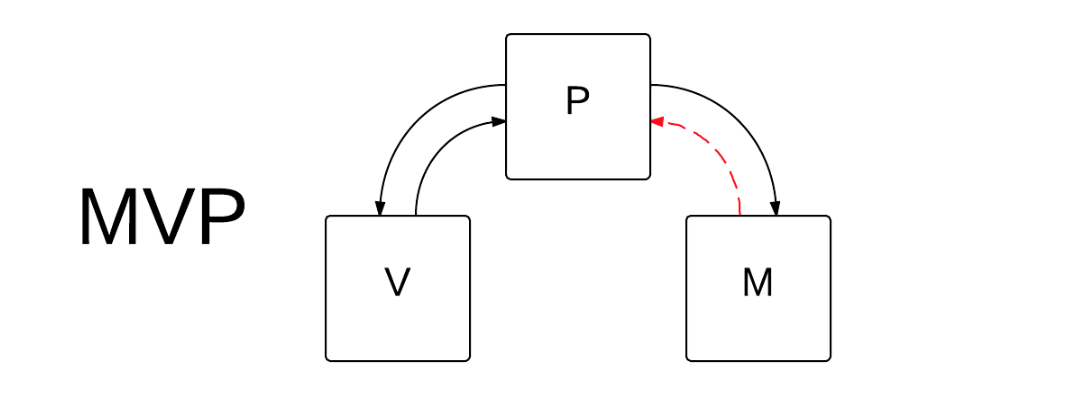
\includegraphics[width=300px, height=100px]{images/mvp.png}
		\end{itemize}
	\end{frame}
	
	
%	\subsection{Design}
%	\begin{frame}{Architecture (Design)}
%		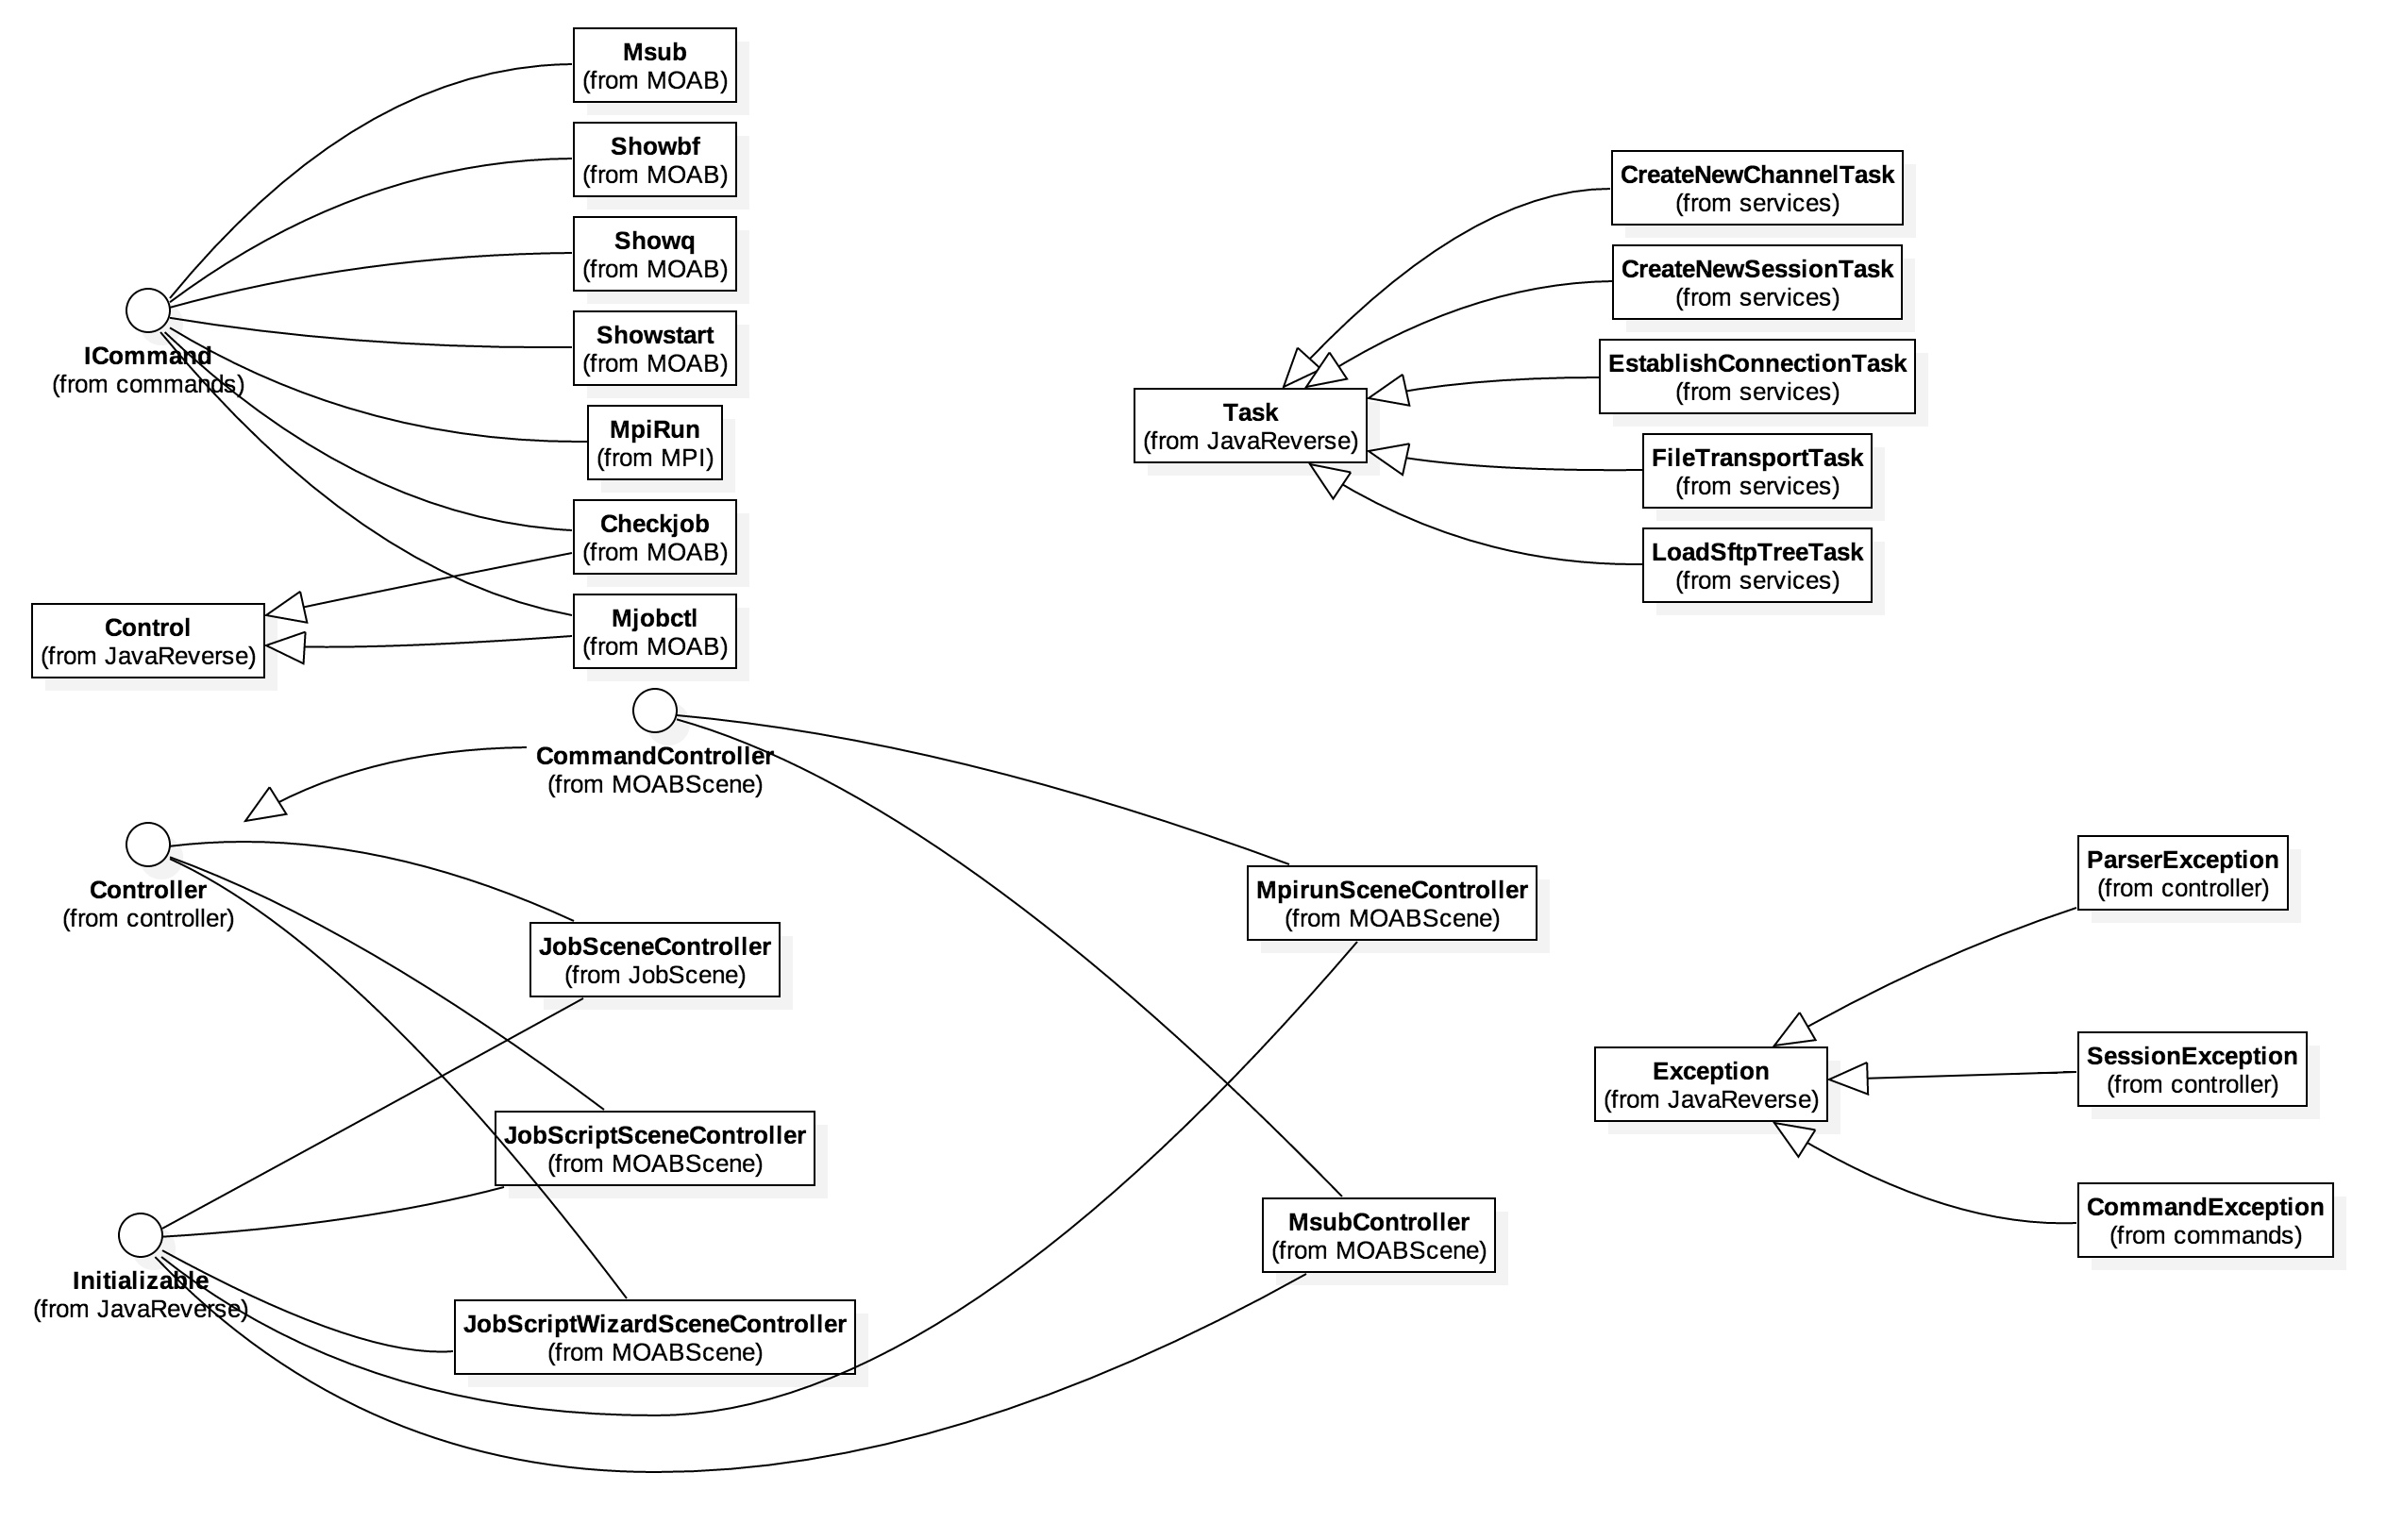
\includegraphics[width=300px, height=210px]{images/GUIDesign.png}
%	\end{frame}
	

	\begin{frame}{GUI: SSH-Connection}
		\begin{tikzpicture}[->,shorten >=1pt,auto,node distance=3cm,thick,main node/.style={ ellipse,draw,font=\sffamily\Large\bfseries}]
 
  \node[main node] (1) {Disconnected};
  \node[main node] (2) [below right of=1]{Connecting};
  \node[main node] (3) [below right of=2] {Ready};
  \node[main node] (4) [above right of=3] {Establishing};
  \node[main node] (5) [above right of=4] {Online};

  \path[every node/.style={font=\sffamily\small}]
    (1) edge [bend right] node[left] {Try Connection} (2)
        
    (2) edge [bend right] node[right] {Connection Failed} (1)
        edge [bend right] node[left] {Valid connecion} (3)
    (3) edge [bend left] node[right] {Initiate connection} (4)
    		
    (4) edge [bend right] node[right] {Initiation failed} (1)
       	edge [bend left] node[right] {Success} (5)
    (5)  edge [bend right] node[above] {Disconnect} (1)
         edge [bend left=90] node[right] {Offline} (3);
	\end{tikzpicture}
	\end{frame}
	
	\begin{frame}{GUI: Script generator}
		Shell script generator for MOAB Workload Manager :
		
		\begin{itemize}
			\pause
			\item Parses msub command
			
			\pause			
			\item Specifies the directory in server using lazy tree 
			 
			\pause
			\item Parses mpirun command
			
			\pause
			\item Parses parameters of the dynamic scheduler
		\end{itemize}
	\end{frame}
	
	
	
	\begin{frame}{GUI: Script generator (Structure)}
		
		\begin{block}{run\_scheduler.sh}
		        \#\#\#\# MOAB commands
		        \newline
		        \newline
				\#MSUB  -q develop\\
				\#MSUB  -l nodes=22:ppn=22\\
				\#MSUB  -l walltime=1000\\
				\#MSUB  -M uxdok@student.kit.edu
				\newline
				\newline
        				\#\#\#\# Directory
				\newline
				\newline
				cd ./Documents
				\newline
				\newline
        				\#\#\#\# MPI commands
        			\newline
        			\newline
				mpirun -np 4 ./myExec -design master-worker -strategy fifo
			
		\end{block}
	\end{frame}
	
	
\begin{frame}{GUI: Outcome}
\begin{itemize}
\item What can we do in the graphical user interface?	
\begin{itemize}
			\pause
			 \item Generate scripts and send them in the server
			 \item Visualize the performance of the program 
			 \item Discover relationships in tasks
\end{itemize}
\pause
\item GUI features are bound to the dynamic scheduler!
\pause
\item  \Frowny{} We are limited to a lot of other great MOAB Workload Manager features
%\begin{itemize}
			
%\item In The Beginning... was the Command Line - Neal Stephenson
%\end{itemize}
\pause
\item \Smiley{} Extensibility - implementation takes future growth into consideration 
	\end{itemize}
		
	\end{frame}
	